\subsection{拟伽罗瓦扩张}

定义 2.——设 E 是 K 的一个扩张。若 E 是代数的，并且 K{[}X{]} 中在 E 里至少有一个根的每个不可约多项式都在 E{[}X{]} 中分解为一些 1 次多项式（未必互异）之积，则称 E （在 K 上）是拟伽罗瓦的或正规的。

若 E 是 K 的一个代数闭包，则它是 K 的拟伽罗瓦扩张；因为命题 1 的条件 (AC)（V，第 19 页）断言 E{[}X{]} 中的每个非常数多项式都是一些 1 次多项式之积。

命题 3.——设 E 是包含在 Ω 中的 K 的一个扩张。则下列条件等价：

\begin{enumerate}
\def\labelenumi{\alph{enumi})}
\item
  E 是 K 的一个拟伽罗瓦扩张。
\item
  对每个 \(x \in \mathbf{E}\) ，\(x\) 在 \(\mathbf{K}\) 上的、位于 \(\Omega\) 中的共轭元都属于 \(\mathbf{E}\) 。
\item
  \(\Omega\) 的每个 K-自同构都把域 E 映到其自身内。
\item
  E 到 \(\Omega\) 中的每个 K-同态都把 E 映到其自身内。
\item
  E 是 \(\Omega\) 中一族非常数多项式 \((f_i)_{i\in I}\) （K{[}X{]} 中的）所确定的分裂扩张（V，第 24 页，注 3）。
\end{enumerate}

c) 与 d) 的等价性源于这样的事实：E 到 \(\Omega\) 中的每个 K-同态都由 \(\Omega\) 的一个 K-自同构诱导（V，第 52 页，命题 1）。

按定义，拟伽罗瓦扩张是其元素的（在 K 上的）极小多项式所成族的分裂域，故 \(a\) 蕴含 \(e\) )。在假设 \(e\) 下，设 \(u\) 是 \(\Omega\) 的一个自同构；对每个 \(i \in I\) ，\(u\) 置换根集 \(\mathbf{R}_i\) （\(f_i\) 的），且由于 \(\mathbf{E} = \mathbf{K}\left(\bigcup_{i \in I} \mathbf{R}_i\right)\) ，我们有 \(u(\mathbf{E}) = \mathbf{E}\) ；于是 \(e\) 蕴含 \(c\) 。

共轭元素的定义表明 \(c)\) 蕴含 \(b)\) 。最后假设 \(b)\) 成立；设 \(f\) 是 \(K[X]\) 中的一个首一不可约多项式，它至少有一个根 \(x\) （\(E\) 中的）；由于 \(\Omega\) 是代数闭的，存在元素 \(a_k\) （\(\Omega\) 的，\(1 \leqslant k \leqslant n\) ）使得 \(f(x) = \prod_{k=1}^{n} (X - a_k)\) ，又由于 \(a_k\) 是 \(x\) 在 K 上的共轭元（V，第 53 页，推论 1），由假设它们属于 E。于是我们证明了 b) 蕴含 a)。

推论 1.——包含在 Ω 中的 K 的扩张 E 是拟伽罗瓦的，当且仅当它与它在 K 上的所有共轭相同。

这由命题 1 的 a)（V，第 52 页）以及命题 3 中条件 \(a\) 与 \(c\) 的等价性得出。

推论 2.——设 E 与 F 是 K 的两个代数扩张，且 \(E \subset F\) 。若 F 在 K 上是拟伽罗瓦的，则它在 E 上也是拟伽罗瓦的。

我们可以假设 \(F \subset \Omega\) 。设 u 是 \(\Omega\) 的一个 E-自同构。由于 u 是 \(\Omega\) 的 K-自同构且 F 在 K 上拟伽罗瓦，我们有 \(u(F) = F\) ，因此 F 在 E 上是拟伽罗瓦的。

推论 3.——设 N 是包含在 \(\Omega\) 中的 K 的一个拟伽罗瓦扩张，E 是 N 的一个子扩张。设 u 是 E 到 \(\Omega\) 中的一个 K-同态；则 \(u(E) \subset N\) ，且存在 N 的一个 K-自同构 v，它在 E 上诱导 u。

设 w 是 \(\Omega\) 的一个延拓 u 的 K-自同构（V，第 52 页，命题 1）；由于 N 在 K 上拟伽罗瓦，我们有 \(w(\mathbf{N}) = \mathbf{N}\) ，从而 \(w(\mathbf{E}) \subset \mathbf{N}\) ，于是 w 诱导出 N 的一个 K-自同构 v。

推论 4.——设 E' 是 K 的一个扩张，E 与 K' 是 E' 的两个子扩张。假设 E 在 K 上是拟伽罗瓦的且 E' = K'(E) ；则 E' 在 K' 上是拟伽罗瓦的。

设 \((f_i)_{i\in I}\) 是 \(\mathbf{K}[\mathbf{X}]\) 中的一族非常数多项式，它们在 \(\mathbf{K}\) 上的分裂域是 E。则显然 \(\mathbf{E}'\) 是该族 \((f_i)_{i\in I}\) 在 \(\mathbf{K}'\) 上的分裂域，故它在 \(\mathbf{K}'\) 上是拟伽罗瓦的。

注.——1) 设 F 是 K 的一个扩张，E 是 F 的一个子扩张，且假设 E 在 K 上是拟伽罗瓦的。我们来证明 F 的每个 K-自同构 u 都保持 E 不变。设 \(x \in E\) ，f 是 x 在 K 上的极小多项式。由于 E 在 K 上拟伽罗瓦，存在 \(a_{1}, \ldots, a_{n} \in E\) 使得 \(f(\mathbf{X}) = \prod(\mathbf{X} - a_{i})\) ；我们有 \(f(u(x)) = u(f(x)) = 0\) ，故 \(u(x)\) 是某个 \(a_{i}\) ，从而属于 E。我们已证明 \(u(\mathrm{E}) \subset \mathrm{E}\) ，再由 V 第 52 页命题 1 即得 \(u(\mathrm{E}) = \mathrm{E}\) 。

\pandocbounded{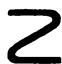
\includegraphics[keepaspectratio]{images/part001_36e9f8fa.jpg}}

\begin{enumerate}
\def\labelenumi{\arabic{enumi})}
\setcounter{enumi}{1}
\item
  设 E 是 K 的一个拟伽罗瓦扩张，F 是 E 的一个拟伽罗瓦扩张；F 在 K 上未必是拟伽罗瓦的（V，第 153 页，例 1）。原因如下：设 u 是 \(\Omega\) 的一个 K-自同构；我们有 \(u(E) = E\) ，但若 f 是 F 的元素 x 在 E 上的极小多项式，它在 u 下未必不变；因此 \(u(x)\) 未必与 x 在 E 上共轭，从而未必属于 F。在这种情形，F 与 \(u(F)\) 是 E 的两个不同的拟伽罗瓦扩张，它们是 K-同构的但不是 E-同构的。
\item
  设 E 是 K 的一个代数扩张，x、y 是 E 的两个元素。若存在 E 的一个 K-自同构把 x 映到 y，则 x 与 y 在 K 上有相同的极小多项式，从而由命题 2（V，第 52 页）在 K 上共轭。若 E 是拟伽罗瓦的，则逆命题成立，因为 \(\Omega\) 的每个 K-自同构都诱导 E 的一个 K-自同构。E 是拟伽罗瓦的这一假设并非多余，如下例所示：设 K = Q，\(\Omega\) 为全体代数数构成的域；令 \(E = \Omega \cap R\) 。可以证明（V，第 153 页，例 2），E 的每个自同构都是恒等映射，且 \(\sqrt{2}\) 与 \(-\sqrt{2}\) 是 E 中在 Q 上共轭的元素。
\end{enumerate}

